\section{Programmazione dinamica}

%

\section{Programmazione greedy}

%

\section{Programmazione lineare}
Spesso è richiesto di massimizzare o minimizzare un determinato obiettivo in base alle risorse disponibili e rispettando alcuni vincoli. In questi
termini parliamo di problemi riconducibili alla \textbf{programmazione lineare} e sono esprimibili come funzioni lineari. Gli algoritmi sui grafi
studiati nel precedente capitolo sono istanze specifiche di questo problema.\par
Introduciamo le dinamiche lavorative con un problema completo: supponiamo di avere una fabbrica di cioccolatini, capace di produrne una tipologia
normale, che frutta un profitto di 1€/scatola, e una tipologia deliziosa, che fa ricavare 6€/scatola. Lo scopo dell'azienda è
produrre le scatole di cioccolatini e massimizzare il prodotto in base ai seguenti vincoli: \begin{itemize}
    \item Sono producibili al massimo 200 scatole al giorno di cioccolatini normali.
    \item Sono producibili al massimo 300 scatole al giorno di cioccolatini deliziosi.
    \item Sono producibili al massimo 400 scatole al giorno.
\end{itemize}

\noindent Provando a riformulare il problema in termini più rigorosi definiamo due variabili $x_1, x_2$ che rappresentano il numero di scatole dei
cioccolatini normali e deliziosi rispettivamente. Inoltre, il profitto massimo sarà dato dalla loro somma. Sapendo ciò, possiamo mettere tutte queste
definizioni a sistema: \[
    \begin{cases}
        x_1 \leq 200\\
        x_2 \leq 300\\
        x_1+x_2 \leq 400
    \end{cases}
\]

\noindent La formulazione del problema in termini di sistema lineare è detta \textbf{formulazione canonica} e rappresenta il punto di partenza per la
risoluzione dei problemi di programmazione lineare. Avendo un sistema, è possibile rappresentarlo graficamente sul piano cartesiano.
\begin{figure}[h]
    \centering
    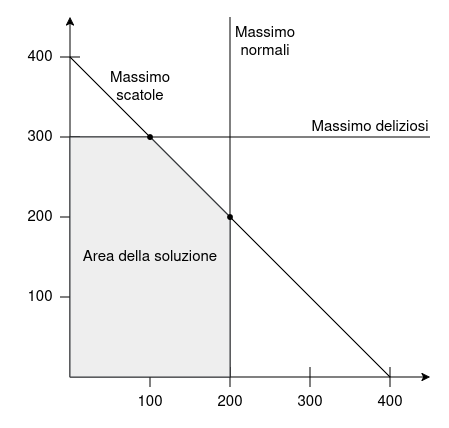
\includegraphics[width=0.7\linewidth]{Images/linearProgramming.png}
    \caption{Grafico del problema}
\end{figure}

\noindent Si può notare che la soluzione è rappresentata da un'area delimitata dalle funzioni lineari del sistema di disequazioni, un politopo convesso
detto \textbf{simplesso} formato da spigoli (il suo perimetro) e vertici (le intersezioni), dove questi ultimi sono le soluzioni del sistema.\par
È possibile costruire una retta che rappresenta tutti i punti per cui la soluzione esiste, il cui valore varia in base alla traslazione. In questi
termini è possibile spostarla per eventualmente ottenere la soluzione massima, traslandola più in alto o minima, traslandola più in basso, a seconda
delle necessità del problema a patto che intersechi la regione ammessa. In questo caso la soluzione è $x_1+6x_2=1900$ ed è evidente, ma si necessita
un algoritmo per la trattazione di casi più complessi.\par
L'\textbf{Algoritmo del simplesso} è utilizzato per l'esplorazione della regione ammessa: prende in input un programma lineare e ne restituisce una
soluzione ottima. Inizia da un vertice del simplesso ed esegue una sequenza di iterazioni, dove in ognuna di loro si sposta lungo un lato della figura
verso un vertice adiacente al corrente tale per cui il valore obiettivo non sia più piccolo di quello attuale. L'algoritmo permina quando è raggiunto
un massimo locale, un vertice i cui vertici adiacenti hanno tutti un valore obiettivo più piccolo. Inoltre, in quanto la regione è convessa e la
funzione obiettivo è lineare, l'ottimo locale diventa un ottimo globale.\par
Generalmente, l'algoritmo del simplesso risolve i problemi di programmazione lineare in tempi polinomiali relativamente rapidi, ma presenta nel caso
peggiore una complessità esponenziale. Inoltre, ragionando in termini di sistemi lineari, è possibile utilizzare le nozioni di algebra lineare a nostro
vantaggio e rappresentarli in forma matriciale. Se applicata al precedente problema, otteniamo la forma
$Ax \leq b$: \[
    A = \begin{pmatrix}
    1 & 0\\
    0 & 1\\
    1 & 1\\
\end{pmatrix}\quad x = \begin{pmatrix}
    x_1\\
    x_2
\end{pmatrix}\quad b = \begin{pmatrix}
    200\\
    300\\
    400
\end{pmatrix}
\]

\noindent E lo scopo del problema diventa trovare il massimo valore $c_x$ tale per cui $c = \left<1, 6\right>$. Aggiungiamo ora un nuovo vincolo al
problema: la produzione di cioccolatini deluxe, per un profitto di 13€/scatola e richiedenti il triplo del materiale dei deliziosi per fare una scatola.
Allora i vincoli del sistema di disequazioni lineare diverrebbero: \[
    \begin{cases}
        x_1\leq 200\\
        x_2\leq 300\\
        x_1+x_2+x_3\leq 400\\
        x_2+3x_3\leq 600
    \end{cases}
\]

\noindent Il valore massimo sarà dato quindi da $x_1+6x_2+13x_3$, e dove il problema sarebbe rappresentabile graficamente in $\mathbb{R}^3$, sarebbe
estremamente dispendioso in termini di tempo. Verifichiamo quindi il risultato grazie a una combinazione lineare dei vincoli: \[
    \begin{pmatrix}
        0(x_1) & 0 & 0 & \vline & 0(200)\\
        0 & 1(x_2) & 0 & \vline & 1(300)\\
        1(x_1) & 1(x_2) & 1(x_3) & \vline & 1(400)\\
        0 & 4(x_2) & 4(3x_3) & \vline & 4(600)
    \end{pmatrix} \implies x_1 + 6x_2 + 13x_3 \leq 3100
\]

\noindent La disequazione è ottenuta sommando i valori di ogni colonna, ed è chiaro che rappresenta la soluzione ottima. Tuttavia abbiamo bisogno di
un qualche metodo per determinare i valori dal moltiplicare agli elementi della matrice. Riprendiamo quindi il problema originale rimuovendo i
cioccolatini deluxe e definiamo i moltiplicatori $y_1, y_2, y_3$ da utilizzare per ricavare la disequazione del vincolo della combinazione lineare.
Dato il sistema in essere, risulterà: \[
    \begin{pmatrix}
    (y_1)x_1 & 0 & \vline & (y_1)200\\
    0 & (y_2)x_2 & \vline & (y_2)300\\
    (y_3)x_1 & (y_3)x_2 & \vline & (y_3)400 
\end{pmatrix} = (y_1+y_3)x_1 + (y_2+y_3)x_2 \leq 200y_1 + 300y_2 + 400y_3
\]

\noindent Se $y_1+y_3 \geq 1$ e $y_2 + y_3 \geq 6$, ovvero sono maggiori o uguali del valore del profitto, la disequazione del vincolo produce un limite
superiore pari a $200y_1 + 300y_2 + 400y_3$, il valore della funzione obiettivo $x_1+6x_2$. Lo scopo è rendere minimo il limite superiore con una scelta
corretta del moltiplicatori, dunque bisognerà trovare il valore minimo del vettore $b = \left<200y_1, 300y_2, 400y_3\right>$. Si tratta di un altro
problema di programmazione lineare con la seguente forma matriciale: \[
    A'y \leq b' = \begin{pmatrix}
        1 & 0 & 1 & \vline & 1\\
        0 & 1 & 1 & \vline & 6
    \end{pmatrix}\quad min(c'y) = \begin{pmatrix}
        200 & 300 & 400
    \end{pmatrix}
\]

\noindent Possiamo notare che il problema iniziale di $Ax \leq b$ è strettamente legato a questo sottoproblema della ricerca del minimo $A'y\geq b'$ con
$min(c'y)$; questo perché $A'=A^T$, ma anche perché $b'=c^T$ e $c'=b^T$. Il primo problema è detto \textbf{primale}, mentre il secondo è il
\textbf{duale}; sono complementari ed è possibile passare da uno all'altro scambiando i vincoli con gli obiettivi. Il secondo problema è utile per
ricavare dei limiti al primo grazie al \textbf{Teorema della dualità forte}, il quale afferma che se il primale ha una soluzione ottima finita, allora
anche il duale ne ha una e i valori ottimi delle due funzioni obiettivo coincidono. Se invece il primale è un problema illimitato, il duale è
inammissibile e viceversa.